This section specifies the software architecture requirements and the software architecture design
for the first level of granularity - the system as a whole. The output will be the high level software
architecture components, the infrastructure between them and the tactics used at the first level of
granularity to realize the quality requirements for the system.
Subsequent sections will focus on the software architecture requirements and design for these
high-level architectural components. Note that many of the architectural requirements (particularly
the quality requirements) will be propagated down to lower level architectural components.

\section{Architecture Requirements}
This section discusses the software architecture requirements around the 
required software infrastructure within which the application functionality is
to be developed. The purpose of this infrastructure is to address the
non-functional requirements. In particular the architecture requirements
specify.
\begin{itemize}
	\item the architectural responsibilities which need to be addressed
	\item the access and integration requirements for the system
	\item the quality requirements
	\item the architecture constraints specified by the client
\end{itemize}
\subsection{Access and Integration Requirements}
\subsubsection{Access Channels}
At the first level of granularity we require one system access channel to
facilitate communication between the management and benchmark client service.

The benchmark client applications or so-called "watcher" applications will upon
completion of there benchmarking jobs need to report the results back to the
management system which will need to further process and persistent the results
upon receiving them. We therefore have require a common access channel or
commom communication medium to faciliate communication between these disparate
systems.

\subsection{Quality Requirements}
This section will specify the quality requirements at the highest level of
granularity. These requirements will propagate throughout the entire system
into every other compopent. Quality requirements that are spesific to certain
parts of the system will be discussed under that system's section.

\subsubsection{Flexibility}
The system should utilize dependency injection, open standard protocols,
open source library implemenations to allow the user to switch out any
realization of a technology with another without any problems. Furthermore
the system must utilize software engineering best practices as far as possible
to allow the system to be easily expanded upon by any member of the public
domain as this project is to released a community open source project.

\subsubsection{Maintainability}
Amongst the most important quality requirements for the system is
maintainability. It should be easy to maintain the system in the future. To this end
\begin{itemize}
	\item Future developers should be able to easily understand the system,
	\item The technologies chosen for the system can be reasonably expected to be available for a long time
	\item Developers should be able to easily and relatively quickly
	\begin{itemize}
		\item Change aspects of the functionality the system provides, and
		\item Add new functionality to the system.
	\end{itemize}
\end{itemize}

\subsubsection{Scalability}
As this system is envisaged to be used in academia and industry, it should allow
for easy scaling, in all layers, allowing one to expand only the layer that is
currently under pressure. This requirements leads to the requirements that the
system itself should be able to handle high amounts of traffic especially on the
enterpeise message bus.

\subsubsection{Reliability}
The system must be reliable in terms of messages exchanged on the message bus
as we would want to avoid a situation where users results get lost in the
system and require users to possible run an expensive experiment a second
time.

\subsubsection{Security}
The messages and message queues should be protected from unauthorized acces
which includes, unauthorized posting or reading of messages to message queues,
unauthorized clustering and broker setup.

Any other components or other access channels, such as replication services, web
interfaces or consoles should be properly protected.

\subsubsection{Auditability}
Each message processed by the messaging infrastructure should be tracable to
the user or system that inserted that message into the message infrastructure.
Optionally, a message's integrity should also be verifable as to ensure the
message was not changed during transit.

\subsubsection{Integrability}
The chosen message infrastructure and lower level components namely the
management system and watcher application should be integrable over a common
interface.

\subsubsection{Deployability}
The system must be buildable from source and build scripts only.
The system must be deployable
\begin{itemize}
	\item on Linux servers,
	\item in environments using different message brokers for the
	enterprise message bus.
\end{itemize}

The system should ultimately be packaged as a series of Docker images which are
deployable as Docker containers installed on virtual or physical Linux servers.

\subsection{Architectural Responsibilities}
The architectural responsibilities of the enterprise service bus are shown in 
Figure \ref{fig:ESBResponsibilities}
\begin{figure}[H]
	\begin{center}
	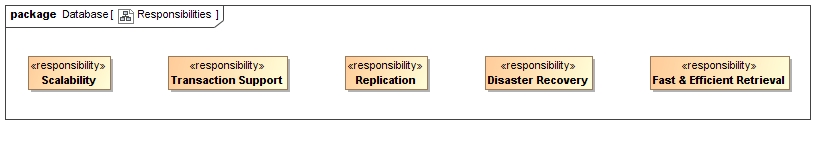
\includegraphics[scale=0.5]{../Diagrams and Charts/Database/Responsibilities.jpg}
	\caption{The architectural responsibilities of the Enterprise Service Bus (ESB)}
	\label{fig:ESBResponsibilities}
	\end{center}
\end{figure}

\subsection{Architecture Constraints}
\label{sec:systemArchitecturalConstraints}
The chosen architecture was determined to best fulfill the non-functional
requirements for the system as well as the requirements set forth by the
client.
\begin{itemize}
	\item The architecture must be deployable on Linux servers
	\item All libraries, frameworks, programming languages and any other
	material of sort utlized within this project must be open-source.
	\item All libraries, frameworks, programming languages and any other
	material of sort used must be supported by open standards, have an 
	active and vibrant support community and should have an active 
	release cycle. 	
\end{itemize}

\subsection{Architecture Design}
\subsubsection{Frameworks and Technologies}
\paragraph{Enterprise Service Bus}
As the benchmark service is based on an enterprise service bus architecture,
the choice of which message bus to use is a critical decision. It was determined
that the Apache ActiveMQ as the implementation. 

Apache ActiveMQ has a vibrant support community, supports various programming
languages, and has a very active release cycle, with the latest stable release
being version 5.13.1 released in February 2016, at this time of this writing.

Features of Apache ActiveMQ includes:
\begin{itemize}
	\item Spring Framework support
	\item Support J2EE servers
	\item Supports pluggable transport protocols
	\item Designed for high performance clustering and client-server communication
	\item Full support for Enterprise Integration Patterns
\end{itemize}

Other implementations considered:
\begin{itemize}
	\item Apache Apollo
	\item Apache Qpid
	\item Pivotal RabbitMQ
\end{itemize}

\subsubsection{Concepts and Constraints for Application Components}
